\documentclass[11pt]{article}

\usepackage[a4paper,margin=2.3cm]{geometry}
\usepackage{graphicx}
\usepackage{booktabs}
\usepackage{amsmath}
\usepackage{amssymb}
\usepackage{xcolor}
\usepackage{enumitem}
\usepackage{caption}
\usepackage[colorlinks=true,linkcolor=blue!60!black,urlcolor=blue!60!black]{hyperref}
\usepackage{titlesec}
\usepackage{fancyhdr}

\definecolor{accent}{HTML}{2b6cb0}
\definecolor{codebg}{HTML}{f5f6f8}

\titleformat{\section}{\Large\bfseries\color{accent}}{\thesection}{0.6em}{}
\titleformat{\subsection}{\large\bfseries}{\thesubsection}{0.5em}{}

\pagestyle{fancy}
\fancyhf{}
\rhead{\small SAkGD --- SA, sa-stress \& the Orchestrator}
\lhead{\small GD 2025 $k$-planarity solver}
\cfoot{\thepage}
\renewcommand{\headrulewidth}{0.3pt}

\newcommand{\code}[1]{\colorbox{codebg}{\texttt{\small #1}}}
\captionsetup{font=small,labelfont=bf}

\title{\vspace{-1.2cm}\textbf{Minimising $k$-Planarity with Simulated Annealing}\\[0.3em]
\large SA, \texttt{sa-stress}, and the Adaptive-Budget Orchestrator}
\author{SAkGD --- Graph Drawing Contest solver}
\date{\today}

\begin{document}
\maketitle
\thispagestyle{fancy}

\begin{abstract}
\noindent This document explains the three layers of the SAkGD solver: (1) the core
\textbf{Simulated Annealing} (SA) engine that moves one node at a time to reduce edge
crossings; (2) \textbf{\texttt{sa-stress}}, which warm-starts SA from a force-directed
layout and is our strongest method on sparse graphs; and (3) the \textbf{orchestrator},
an adaptive scheduler that spends a fixed wall-clock budget across many graphs to
minimise the worst $k$. The solver is a from-scratch re-implementation of the GD~2025
winning approach (Bianchetti \& Moalic, \emph{Winning the GD Challenge for the 4th
Time}) plus our own additions.
\end{abstract}

\section{The problem}
Given a graph, place every node at an \emph{integer} coordinate on a fixed grid so that
(i)~no two nodes share a point and (ii)~no node lies on the interior of an edge it does
not belong to. Edges are drawn as straight line segments. The objective is to minimise
\[
  k \;=\; \max_{e \in E}\; \bigl(\text{number of edges crossing } e\bigr),
\]
i.e.\ the maximum number of crossings on \emph{any single} edge. Ties are broken by the
\emph{total} crossing count $C=\tfrac12\sum_e \mathrm{xc}[e]$. Lower $k$ means a
``more planar'' drawing; a planar graph achieves $k=0$.

\paragraph{Shared engine.} All methods sit on one incremental core:
\begin{itemize}[leftmargin=1.3em,itemsep=1pt]
  \item \textbf{Incremental crossing count.} A node move is scored without a global
  recount --- only edges incident to the moved node and their crossing partners are
  updated (\code{planMove}/\code{commitMove}). The per-edge crossing sets $\mathrm{xs}[e]$,
  counts $\mathrm{xc}[e]$, the histogram $\mathrm{cntPerK}[k]$ and $k$ itself are all
  maintained incrementally.
  \item \textbf{Spatial grid index.} Edges are bucketed into the cells their bounding
  box spans; crossing tests only run against edges sharing a cell.
  \item \textbf{Validity guard.} An \code{occupied} map forbids coincident nodes and a
  fast vertex-edge overlap test forbids a node landing on an edge it is not part of.
\end{itemize}

\section{Simulated Annealing (SA)}
SA follows Algorithm~1 of the paper and runs in \textbf{two phases}, each with its own
fitness function and cooling parameters.

\subsection{Two phases}
\begin{description}[leftmargin=0em,itemsep=2pt]
  \item[\textnormal{\textbf{Phase 1 --- minimise total crossings.}}] Fitness is the
  change in total crossings $\Delta C$. A worsening move ($\Delta C>0$) is accepted with
  the Metropolis probability $\exp(-\Delta C/T)$. This phase does the coarse untangling.
  \item[\textnormal{\textbf{Phase 2 --- minimise the $k$-value.}}] A dual-level fitness:
  the \emph{primary} term is the change in the \emph{local} maximum crossing count among
  the incident edges and their crossing partners; the \emph{tie-breaker} is the
  normalised change in total crossings. This phase specifically attacks the
  bottleneck edges that set $k$.
\end{description}

\subsection{Move proposal and the wave structure}
Each step proposes moving one node:
\begin{itemize}[leftmargin=1.3em,itemsep=1pt]
  \item \textbf{Node selection} (\code{selectNode}) is biased toward nodes touching
  heavily-crossed edges, weight $\approx 1+\sum \mathrm{xc}[e]$.
  \item \textbf{Position selection} (\code{selectPlace}) samples a Gaussian around the
  current position with $\sigma \propto \sqrt{T/T_0}$, plus a 5\% chance of a global
  random jump in Phase~1.
  \item \textbf{Waves.} The run is divided into \emph{waves}. At the start of each wave
  the layout is restored to the best-known solution and the temperature is clipped by
  $decTW$. This lets the search cool, explore, then relaunch from the incumbent best ---
  the sawtooth in Figure~\ref{fig:cooling} (left).
\end{itemize}

The temperature decays geometrically by $decT$ every step and is reset per wave by
$decTW$. As $T$ falls, the acceptance probability of any worsening move collapses
(Figure~\ref{fig:cooling}, right): early on the search wanders freely; late on it behaves
like greedy hill-climbing.

\begin{figure}[ht]
  \centering
  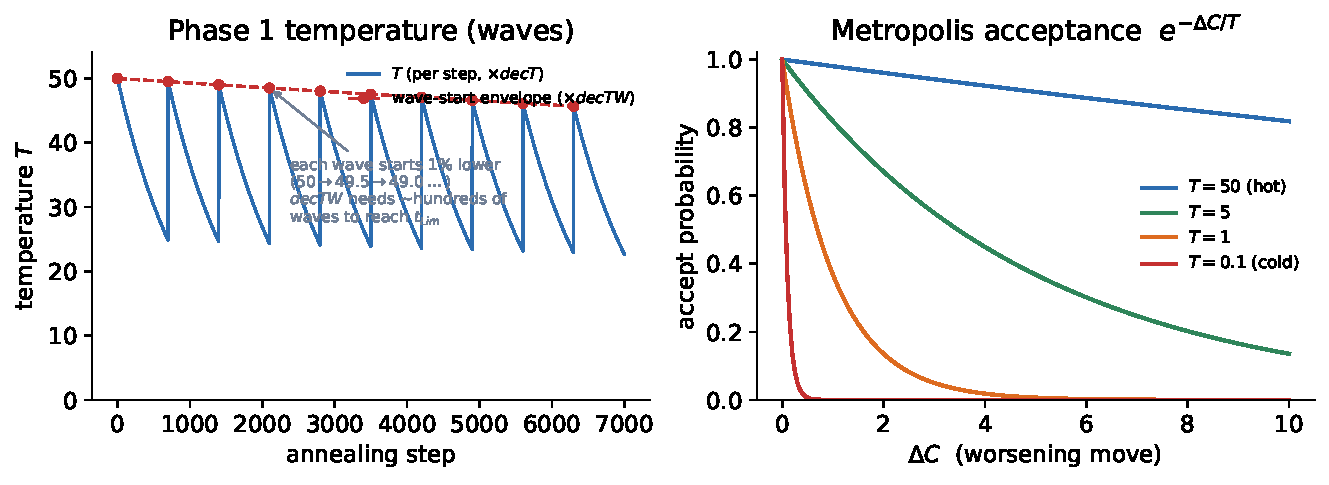
\includegraphics[width=\textwidth]{fig_cooling.pdf}
  \caption{\textbf{Left:} the wave-based temperature schedule for Phase~1
  ($T_0{=}50$, $decT{=}0.999$, $decTW{=}0.99$). Two decays act at once: \emph{within} a
  wave the temperature free-falls as $T\!\times\!decT$ every step (blue); \emph{between}
  waves only the wave-\emph{start} temperature drops, by $decTW$ (red envelope). Because
  $decTW$ is just a 1\% cut per wave, the peaks barely move --- it takes hundreds of waves
  to reach $t_{Lim}$, which is what ends the phase. \textbf{Right:} the Metropolis
  acceptance curve $e^{-\Delta C/T}$ --- hot temperatures accept large worsening moves,
  cold temperatures reject almost everything.}
  \label{fig:cooling}
\end{figure}

\begin{table}[ht]
  \centering
  \caption{SA cooling parameters (paper Table~1).}
  \begin{tabular}{lccccc}
    \toprule
    Phase & objective & $T_0$ & $decT$ & $decTW$ & $t_{Lim}$ \\
    \midrule
    1 & total crossings $\Delta C$ & 50 & 0.999  & 0.99 & 0.01 \\
    2 & $k$-value (local max)      & 1  & 0.9999 & 0.99 & 0.01 \\
    \bottomrule
  \end{tabular}
\end{table}

\section{\texttt{sa-stress}: force-directed initialisation + SA}
SA is only as good as where it starts. The single largest improvement over the baseline
came from replacing the constructive BFS-snake initial layout with a
\textbf{force-directed / stress-minimisation} layout. This is the paper's step~1 (stress
majorization + repeated FMMM, keep the best candidate) rebuilt \emph{without} OGDF ---
whose Python bindings do not work on macOS --- using the Graphviz CLI instead.

\texttt{sa-stress} runs two stages, warm-chained:
\begin{enumerate}[leftmargin=1.4em,itemsep=2pt]
  \item \textbf{\code{tools/stress\_init.py}} ($\approx$8\% of budget). Runs Graphviz
  \textbf{sfdp} (multilevel force-directed, the FMMM analogue) and, on small graphs,
  \textbf{neato} (stress majorization, the SM analogue), up to 8 attempts. Each attempt
  is randomly rotated, scaled to the grid, snapped to integers (collisions pushed to the
  nearest free cell by a spiral search), and scored by a \emph{sampled} crossing density
  ($\sim$200k random edge pairs via NumPy). The best candidate is written. For $n>3000$
  only sfdp is used (faster and consistently better in our experiments).
  \item \textbf{\code{sakgd}} (remaining $\approx$92\%). The two-phase SA above,
  warm-started from the stress layout. If the init stage fails, the BFS-snake safety net
  takes over automatically.
\end{enumerate}

\paragraph{When it helps --- and when it hurts.} On \emph{sparse} graphs (A7/A8/A9,
$m/n\approx2\text{--}3.5$, near-planar densities) a good global embedding drops $k$ by
$3\text{--}4\times$ before SA even starts; SA only polishes. On the \emph{dense} graph A6
($m/n=15$) stress init actually \emph{hurts} --- there is no low-crossing embedding to
find, and the force layout starts worse than a plain random/BFS start
(Figure~\ref{fig:stress}). For dense graphs the orchestrator therefore falls back to
plain \texttt{sa}.

\begin{figure}[ht]
  \centering
  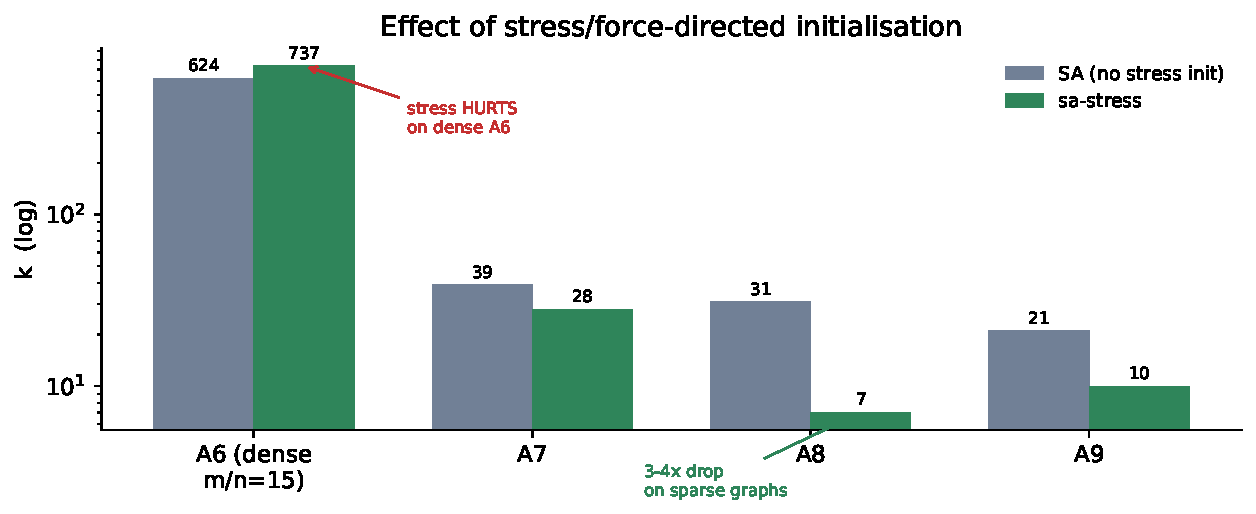
\includegraphics[width=0.86\textwidth]{fig_stress.pdf}
  \caption{Stress/force-directed initialisation collapses $k$ on sparse graphs but
  regresses on the dense A6 (note the log scale). This is why method choice is
  density-dependent.}
  \label{fig:stress}
\end{figure}

\begin{figure}[ht]
  \centering
  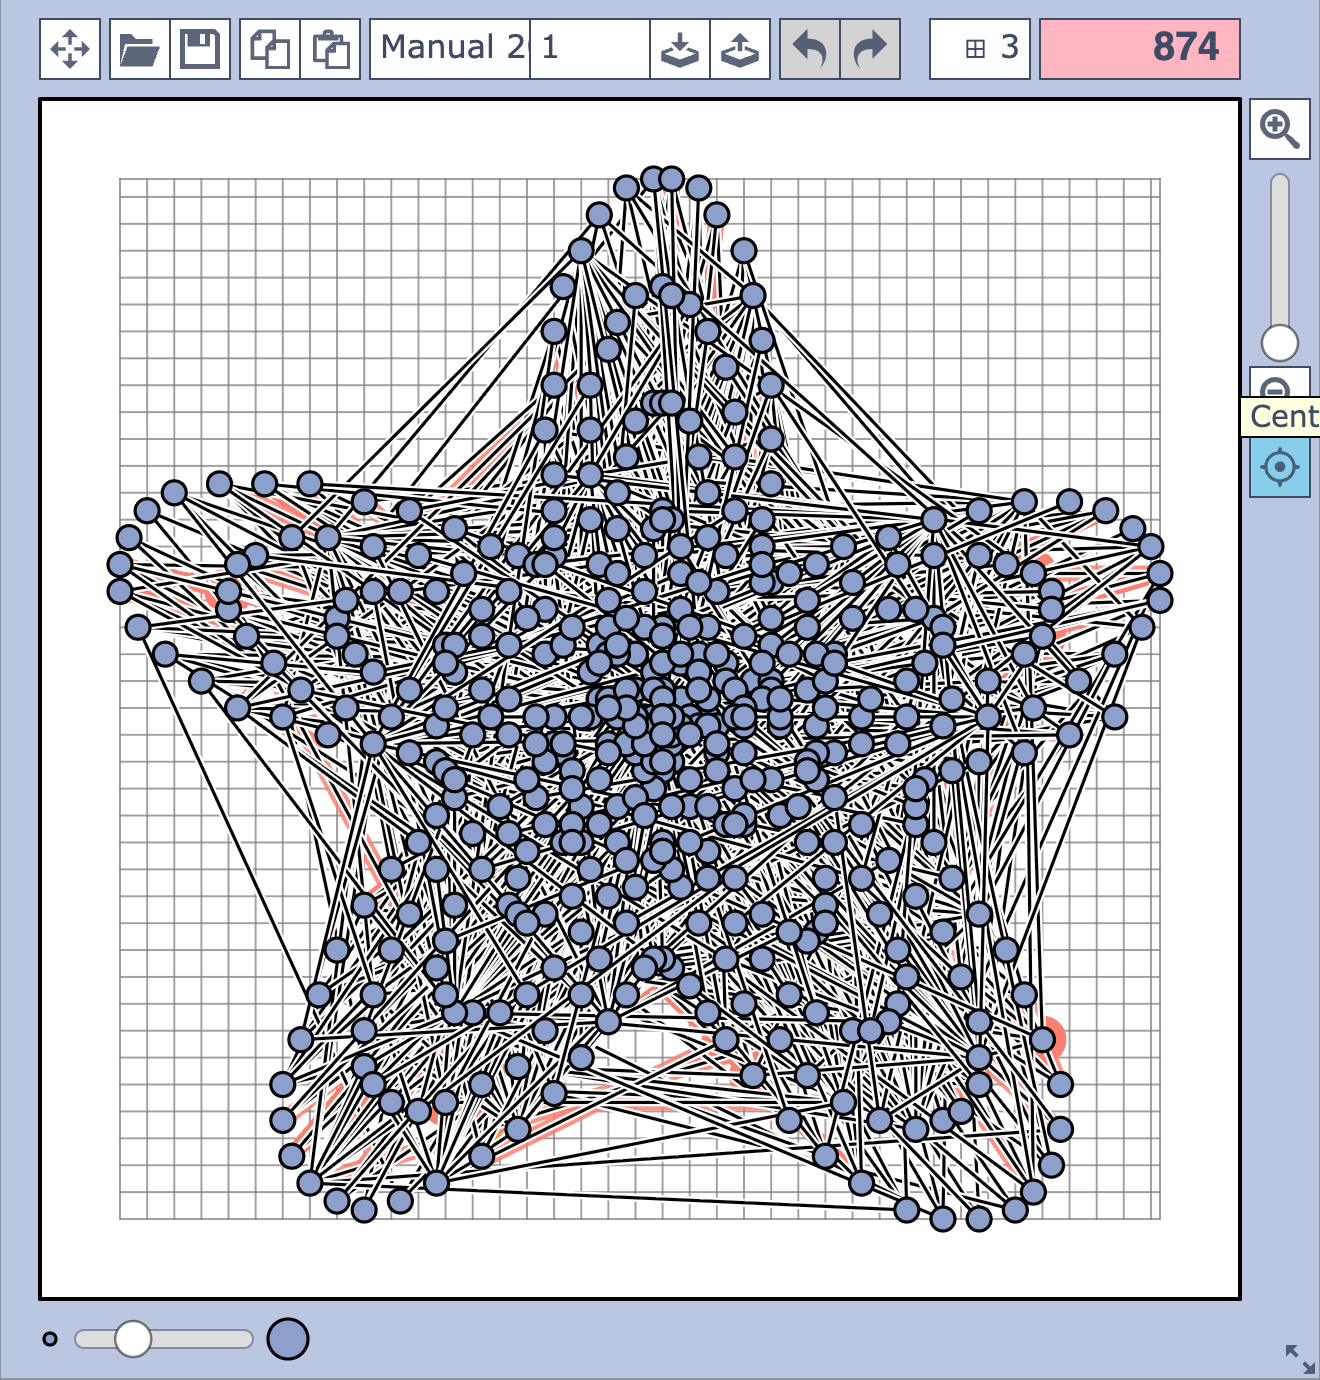
\includegraphics[width=0.245\textwidth]{../phase-screenshots/A7_0_original.png}\hfill
  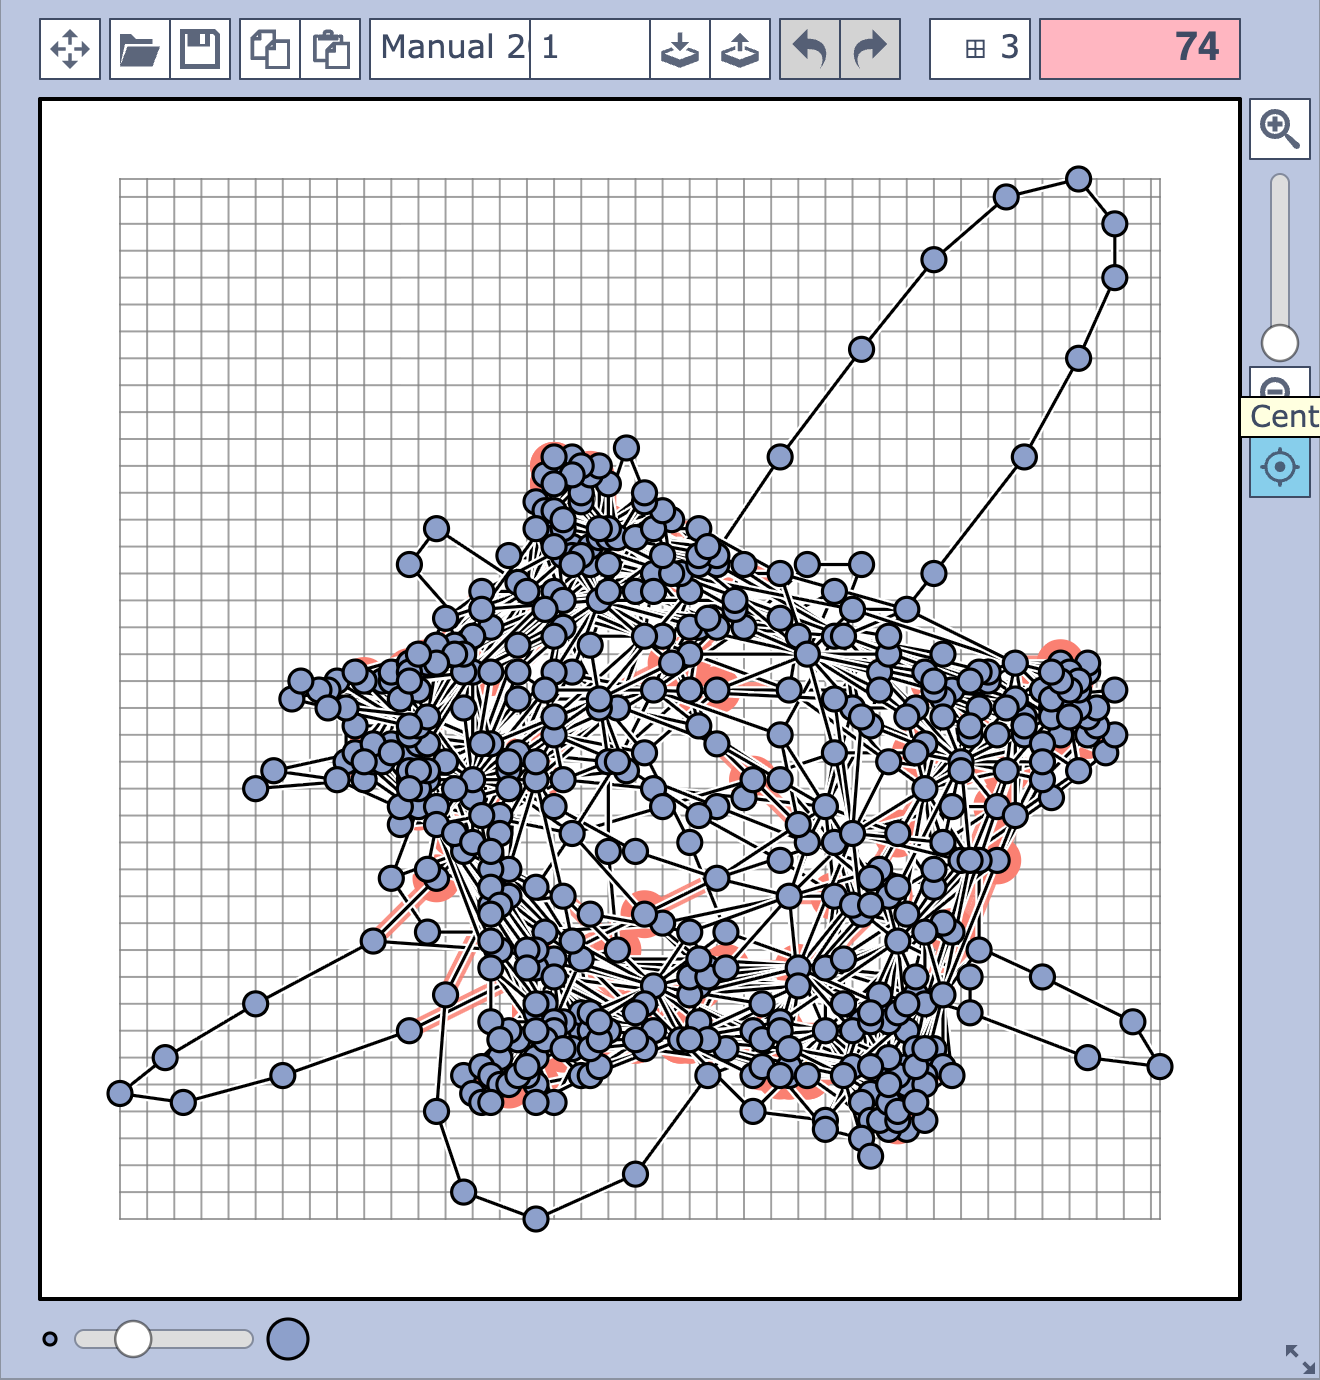
\includegraphics[width=0.245\textwidth]{../phase-screenshots/A7_1_stress.png}\hfill
  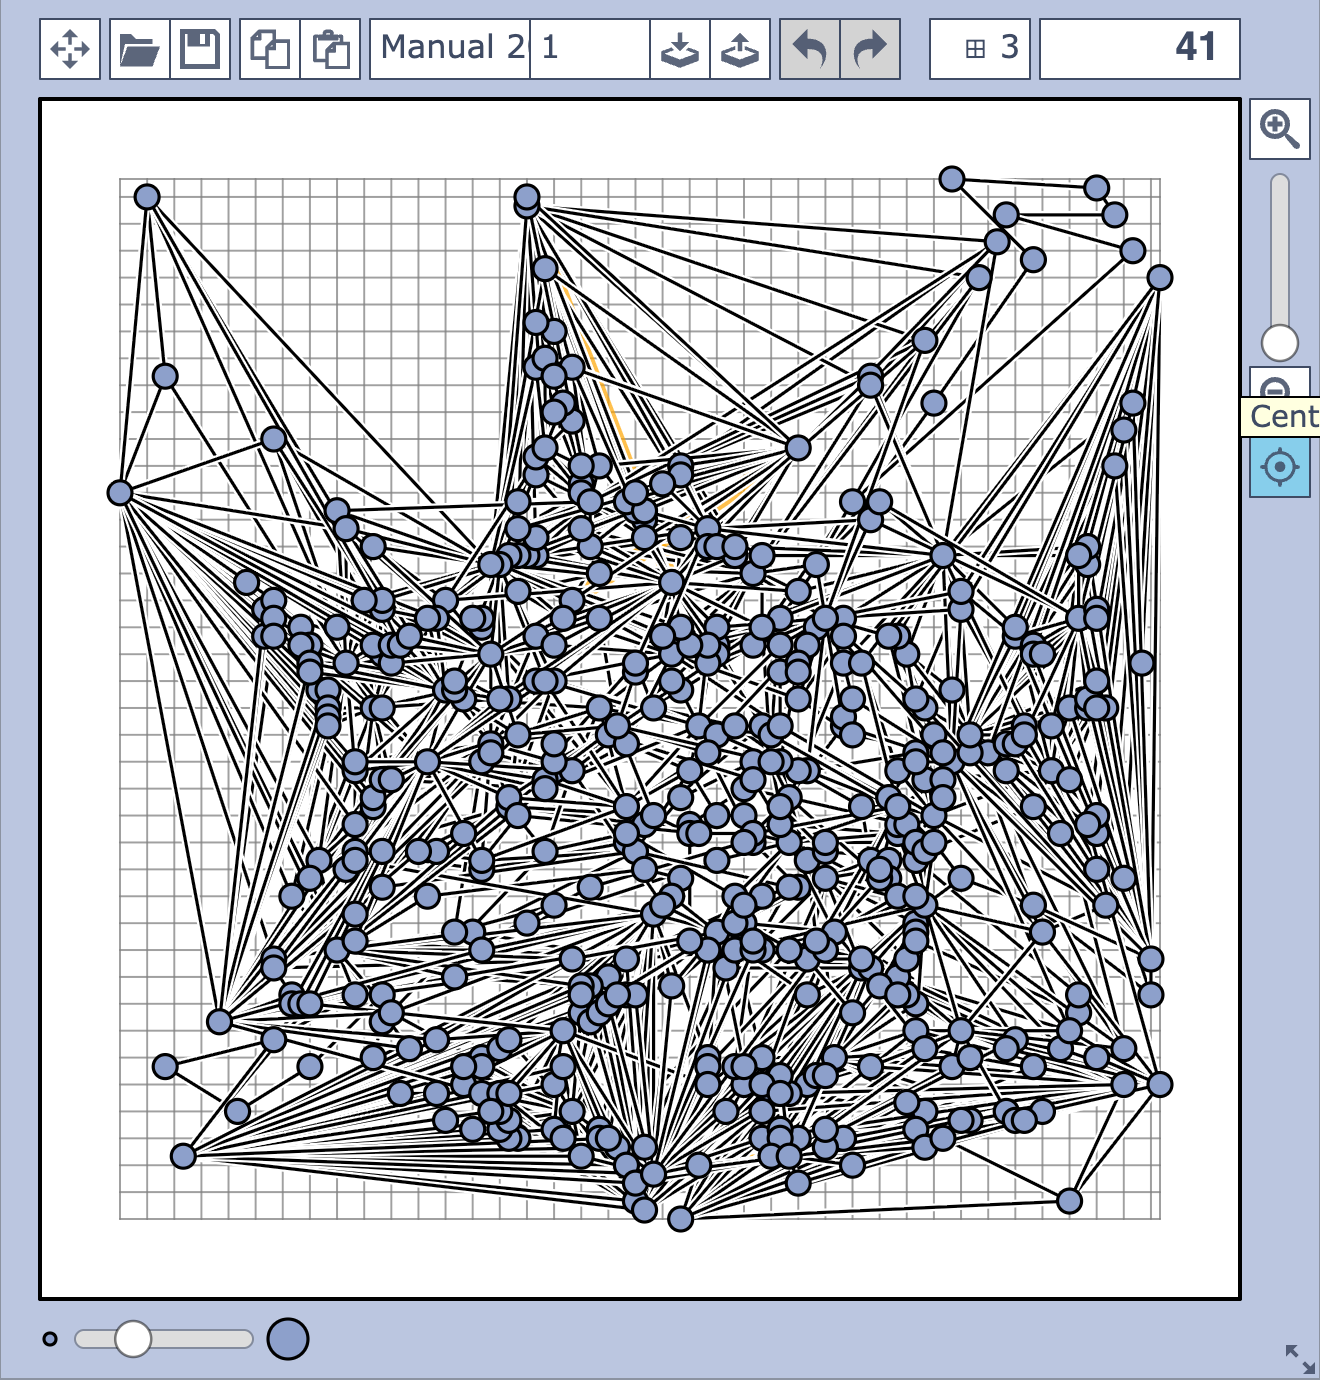
\includegraphics[width=0.245\textwidth]{../phase-screenshots/A7_2_phase1.png}\hfill
  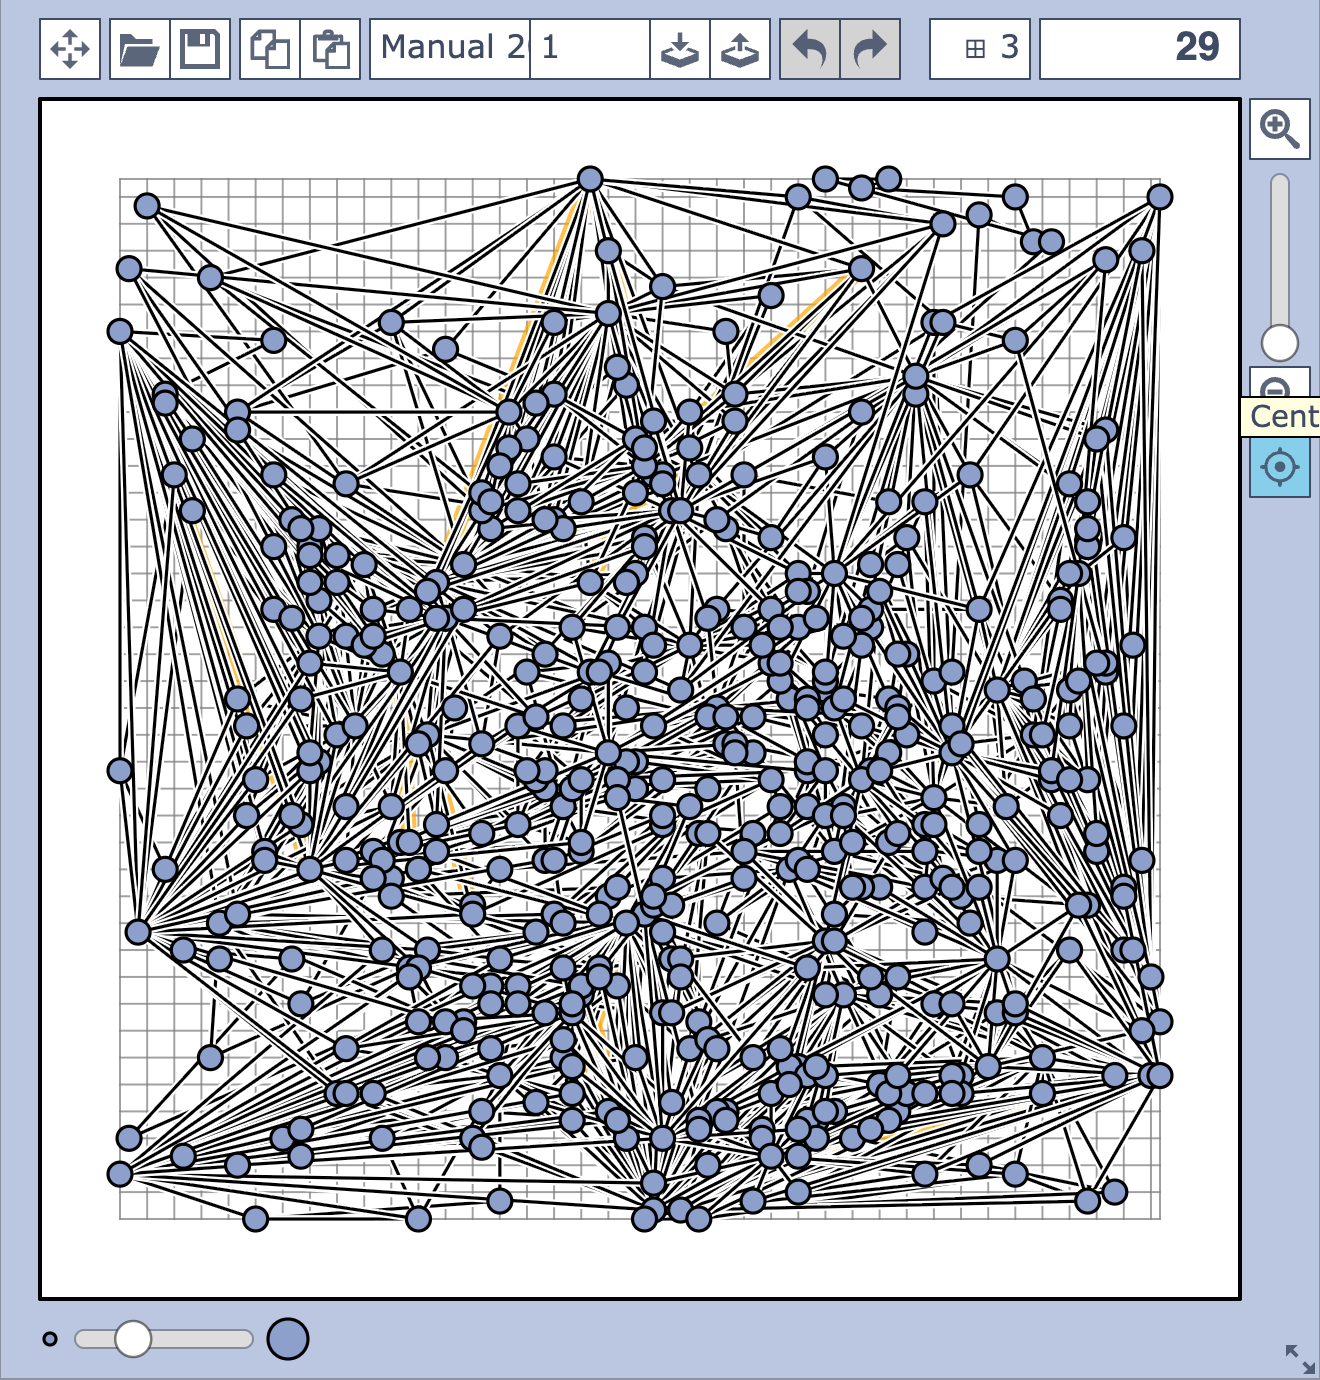
\includegraphics[width=0.245\textwidth]{../phase-screenshots/A7_3_phase2.png}
  \caption{The \texttt{sa-stress} pipeline on Automatic-7, left to right:
  \textbf{(1)} raw input layout, \textbf{(2)} after stress/sfdp initialisation,
  \textbf{(3)} after SA Phase~1 (total-crossing reduction), \textbf{(4)} after SA
  Phase~2 ($k$-value reduction, the final drawing).}
  \label{fig:pipeline}
\end{figure}

\section{Other methods in the portfolio}
Besides \texttt{sa} and \texttt{sa-stress}, the batch runner registers alternative
metaheuristics (the paper uses SA only):
\begin{itemize}[leftmargin=1.3em,itemsep=1pt]
  \item \textbf{\texttt{lns}} --- Large Neighbourhood Search: moves a BFS-connected
  \emph{group} of $K$ nodes per iteration, trying $R$ candidate positions each and
  committing only strictly-improving moves. Escapes some local optima but stalls at a
  local optimum (it never accepts a worsening move).
  \item \textbf{\texttt{ils}} --- Iterated Local Search: alternates a full two-phase SA
  run with a random \emph{kick} that relocates $\sim n/10$ nodes, keeping the global
  best. Directly addresses the LNS stall.
  \item \textbf{\texttt{staged}} --- LNS for 30\% of the budget (fast coarse descent)
  then SA warm-started on that output for the remaining 70\%.
\end{itemize}
After stress-init was added these lost most of their edge, but they remain in the
portfolio. Two literature-backed ideas (\code{--lexk}, \code{--krepair}) were tested,
lost in ablation, and are kept behind default-off flags.

\section{The adaptive-budget orchestrator}
\code{orchestrate.py} answers a different question: given \emph{one} wall-clock budget
(e.g.\ 1 hour) and 8--10 graphs, how do we spend it to minimise the \emph{worst} $k$
across all of them? Spending equal time per graph is wasteful --- some graphs converge in
seconds while others (dense A6) keep improving for the whole hour. The orchestrator is a
\textbf{marginal-gain scheduler}: it measures how fast each graph is still improving and
pours time into whichever graph has the steepest slope.

\subsection{How it works}
\begin{description}[leftmargin=0em,itemsep=3pt]
  \item[\textnormal{\textbf{Classify.}}] From $(n,m)$ pick a method per graph:
  dense/expander ($m/n\ge8$) $\to$ \texttt{sa}; sparse/huge $\to$ \texttt{sa-stress};
  Graphviz-missing $\to$ \texttt{sa}. These thresholds are \emph{soft, CLI-overridable}
  priors that bias only the cold-lease init --- never the scheduler itself.
  \item[\textnormal{\textbf{Quantum leasing.}}] Time is handed out in quanta
  $Q_b=\mathrm{clamp}(B/(4\,n_{\text{live}}),\,45,\,180)$~s via the existing
  $W$-worker multi-start \code{run\_combo}. Huge graphs get a longer floor and fewer
  workers on their first (cold) lease to relieve memory pressure.
  \item[\textnormal{\textbf{Explore.}}] Each graph gets one quantum, hardest-first, so
  every graph yields a real $\mathrm{d}k/\mathrm{d}t$ slope and the huge graph pre-pays
  its expensive setup. Explore is capped at 40\% of the budget $B$.
  \item[\textnormal{\textbf{Convergence / early termination.}}] The best-of-workers
  envelope is read from each graph's \code{.trace}. A graph is dropped when its
  $k$-slope is 0 \emph{and} total crossings fell $<0.5\%$ over a $\ge150$~s window (with
  minimum-lease/tick guards). Hard-drop on $k{=}0$ or temperature floor. Convergence is
  decided purely from the measured trace --- no graph-class exemptions.
  \item[\textnormal{\textbf{Reallocation.}}] Banked time goes to the top bidder,
  $\mathrm{bid}=(\mathrm{d}k/\mathrm{d}t)\cdot Q$, via a \emph{warm-chained} lease
  (\texttt{sa-warm}: a single \code{sakgd} stage with \code{--init input}) resuming the
  graph's verified best layout. Anti-starvation serves the least-serviced among close
  bidders; a minimax sink targets the worst-$k$ graph when nobody improves.
  \item[\textnormal{\textbf{Budget safety.}}] A deadline-aware per-process timeout
  guarantees no lease runs past budget; every graph gets a verified submission (falling
  back to its valid input if needed).
\end{description}

\begin{figure}[ht]
  \centering
  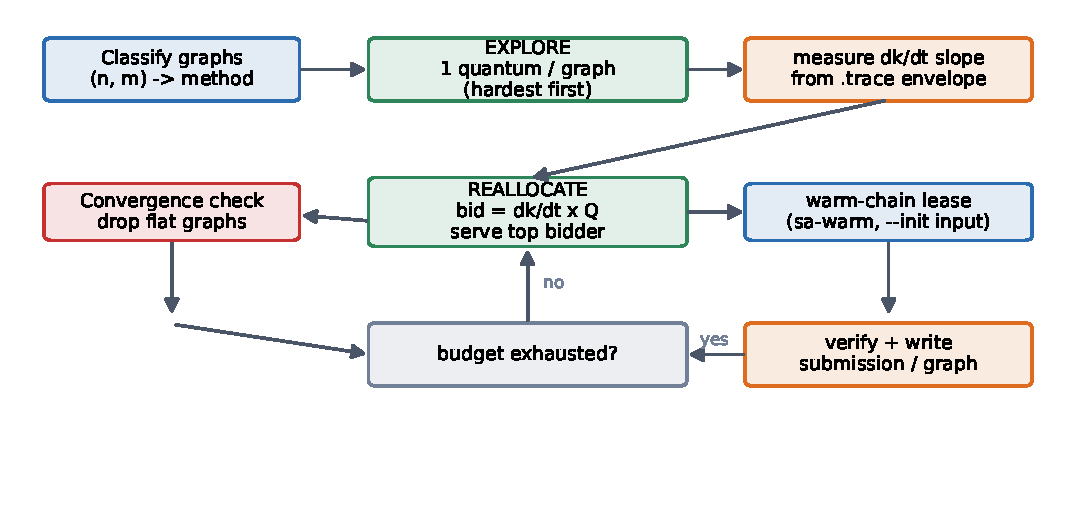
\includegraphics[width=\textwidth]{fig_flow.pdf}
  \caption{The orchestrator loop: explore once per graph to measure slopes, then
  repeatedly reallocate banked time to the steepest-improving graph via warm-chained
  leases, dropping graphs that have gone flat, until the budget is exhausted.}
  \label{fig:flow}
\end{figure}

\subsection{Why warm-chaining is cheap}
A key empirical fact makes this work: resuming a \emph{good} layout with
\code{--init input} is cheap even on the 10k-node A8 --- \code{computeAllCrossings} scales
with the \emph{current} crossing count, not the node count, so a warm continuation of a
$k{=}6$ layout costs $\sim$3~s of setup. Only the raw, tangled input is expensive. Hence
every lease after the first is a cheap, monotone continuation
(Figure~\ref{fig:warmchain}). A killed \code{sakgd} writes no output, so the scheduler
never kills a worker --- the per-lease timeout is only a budget backstop, and a lost
quantum simply keeps the previous warm layout.

\begin{figure}[ht]
  \centering
  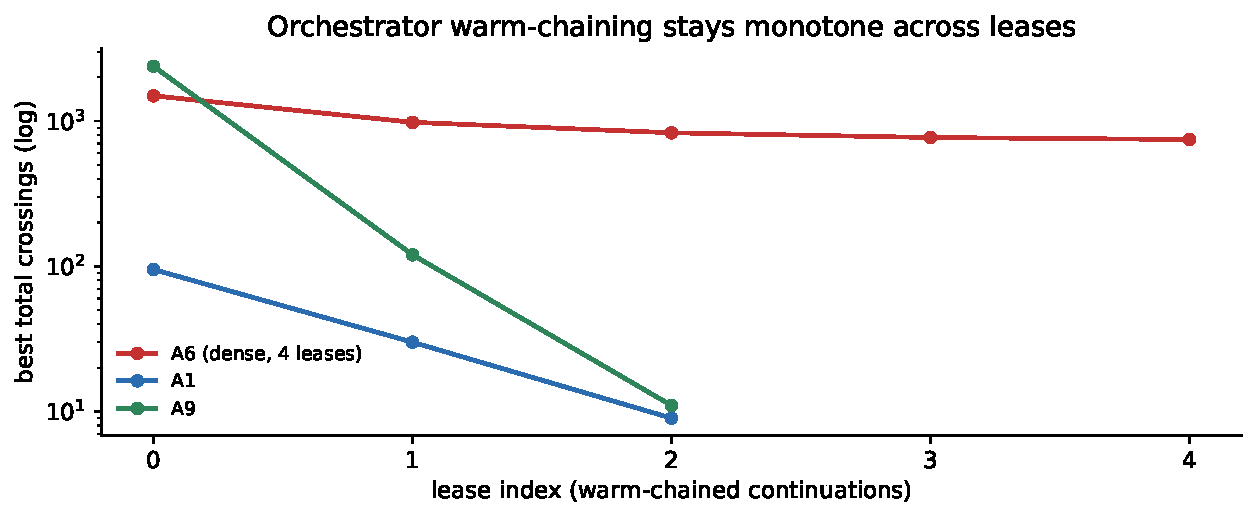
\includegraphics[width=0.86\textwidth]{fig_warmchain.pdf}
  \caption{Warm-chained leases stay monotone (data from a $B{=}220$~s end-to-end run).
  The dense A6 measured as still-improving and won the most budget (4 leases); the
  sparse graphs converged fast and were deprioritised.}
  \label{fig:warmchain}
\end{figure}

\section{Results}
Table~\ref{tab:results} and Figure~\ref{fig:results} summarise the current best $k$ per
contest graph. On the sparse graphs the wins come almost entirely from stress
initialisation (A8: $31\!\to\!7$, A9: $21\!\to\!10$, A7: $39\!\to\!28$), beating both the
rival team and the GD'25 winner. On the dense A6, where stress init does not help, the
only effective lever is budget, and the orchestrator's job is to direct that budget there.

\begin{table}[ht]
  \centering
  \caption{Best $k$ per graph. Lower is better; \textbf{bold} = our current best.}
  \label{tab:results}
  \begin{tabular}{lccccc}
    \toprule
    Graph & $n\,/\,m$ & our old best & \textbf{our new best (method)} & rival & GD'25 winner \\
    \midrule
    Automatic-6 & 200 / 3000     & 632 & \textbf{624} (sa, 15\,min)   & 621 & 568 \\
    Automatic-7 & 500 / 1740     & 39  & \textbf{28} (sa-stress)      & 31  & 31  \\
    Automatic-8 & 10466 / 20288  & 31  & \textbf{7} (sa-stress)       & 12  & 15  \\
    Automatic-9 & 2519 / 4938    & 21  & \textbf{10} (sa-stress)      & 13  & 12  \\
    \bottomrule
  \end{tabular}
\end{table}

\begin{figure}[ht]
  \centering
  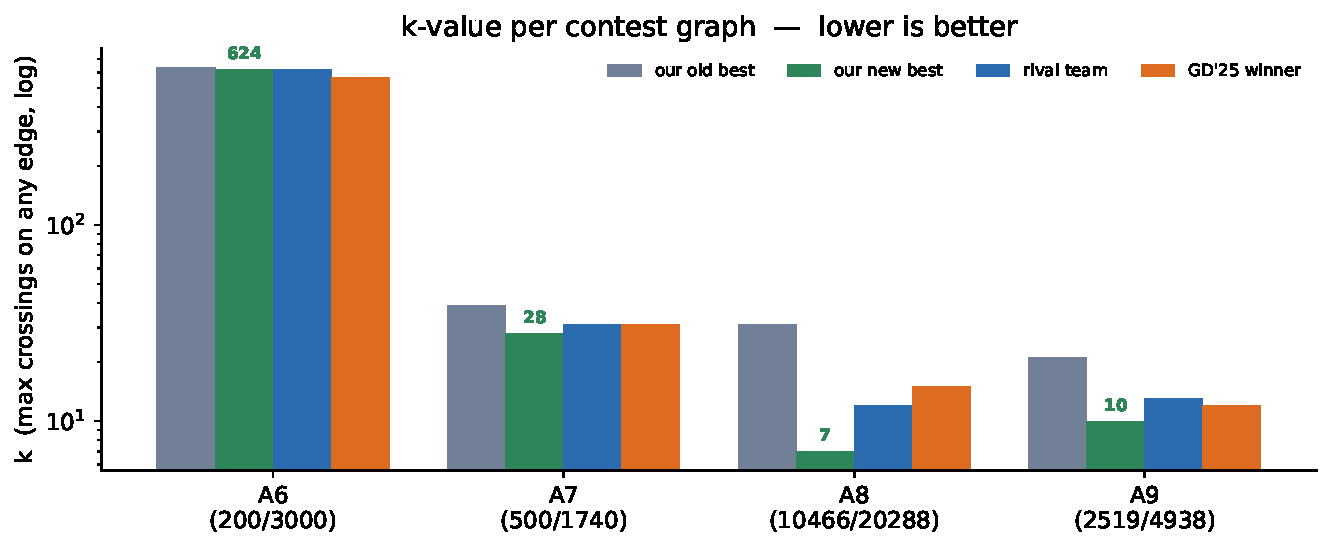
\includegraphics[width=\textwidth]{fig_results.pdf}
  \caption{$k$-value per graph across four solvers (log scale). Our new bests (green) beat
  the rival and the GD'25 winner on all three sparse graphs; A6 remains the open
  frontier.}
  \label{fig:results}
\end{figure}

\subsection*{Quick usage}
\begin{itemize}[leftmargin=1.3em,itemsep=1pt]
  \item Single sparse graph: \code{python3 tools/stress\_init.py -i g.json -o init.json};
  \code{./sakgd -i init.json -o out.json -t 15 -p1 4 --init input}
  \item Full portfolio: \code{python3 run\_contest.py --methods sa-stress,sa --graphs 6-9 --workers 8}
  \item Adaptive 1-hour run: \code{python3 orchestrate.py --graphs 1-9 --budget 3600 --workers 8}
\end{itemize}

\vspace{0.5em}
\noindent\rule{\linewidth}{0.3pt}\\[0.3em]
{\small Reference: Bianchetti, J. \& Moalic, L. (2025). \emph{Winning the GD Challenge for
the 4th Time: Our Approach.} GD~2025, LIPIcs.GD.2025.43. See also
\code{docs/YAKLASIMLAR.md} and \code{results/exp-2026-06-16-orchestrator.md}.}

\end{document}
